\section{Learning-Based Recognition of Human-Grasped Objects}

\subsection{Proposed Approach}
\label{subsection:proposal_overview}

% The adopted solution  focuses on detecting and tracking the hand and finger keypoints from visual data. 
This work proposes a learning-based framework to enable an assistive robot to recognize the object grasped by the human operator. As illustrated in \autoref{fig:LearningFramework}, the proposed framework combines the strengths of MediaPipe in detecting hand landmarks in a RGB image with a deep multi-class classifier that predicts the object based on the configuration of the user’s hand after grasping it. Accordingly, the developed object recognition system operates based on different principles, including the sensing device, the tracking method, and the machine learning approaches. From the point of view of the application in industrial settings, the proposed system has two strengths when compared to the use of data-gloves or electromagnetic motion capture systems. First, the simplicity of installation is associated with a much less complex and costly setup. Second, the non-intrusiveness of the required setup is a valuable factor in accelerating the acceptance of these technologies by humans in carrying out collaborative tasks (a process also referred to as "user adoption"). In contrast, vision-based hand tracking is affected by occlusions, changes in light conditions, and cluttered backgrounds. Furthermore, these problems are difficult to overcome with deep-learning techniques given the data dependency and generalization problems against hands, objects, and lighting conditions outside the training sets. Overall, this paper contributes to advances in understanding the opportunities and limitations of using this novel approach for the recognition of human-grasped objects.

\begin{figure}[ht]
    \centering
    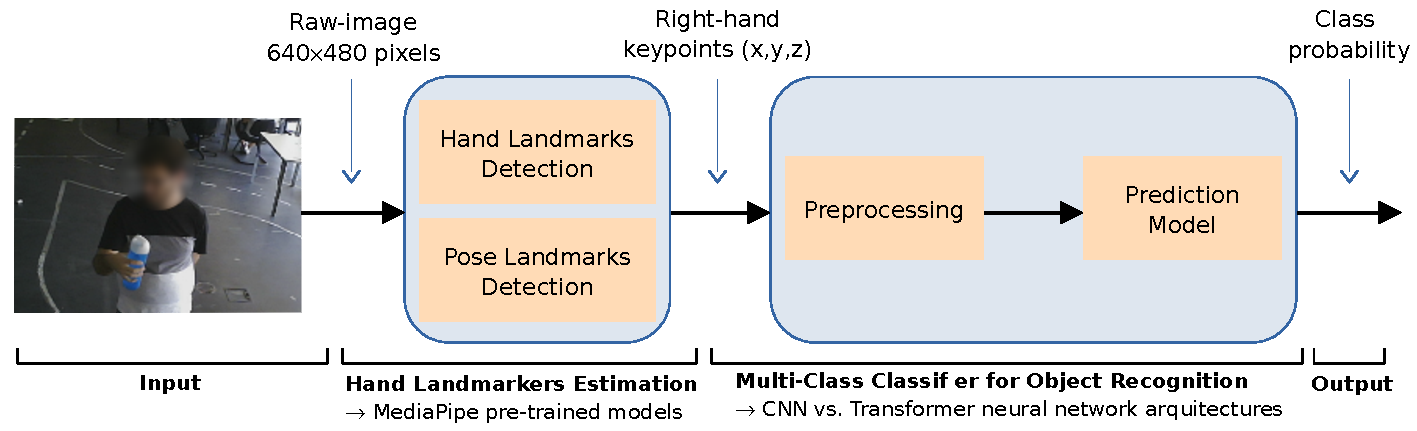
\includegraphics[width=1\columnwidth]{figs/LearningFrameworkB.pdf}
    \caption{The proposed learning-based framework for object recognition based on the hand keypoints.}
    \label{fig:LearningFramework}
\end{figure}

The output of the pre-trained model provides the $(x,y,z)$ coordinates of landmarks for each detected hand. The $(x,y)$ coordinates represent the horizontal and vertical positions of the landmark on the image plane, while the $z$-coordinate represents an estimate of the relative depth with respect to the wrist reference \cite{Amprimo2023}. This work focuses on tracking the right hand by combining the Hand Landmark detection and the Pose Landmark Detection pre-trained models. This strategy proved to be useful to enhance the reliability of the process of extracting the coordinates of the right-hand keypoints from each frame.

The multi-class classifier for object recognition faces several challenges. First, there is limited information about the three-dimensional configuration of the hand, namely if the hand configurations involve overlapping fingers or positions close to each other in the image plane. Consequently, the $z$-coordinate (relative depth) revealed to be a critical element for discriminating complex hand configurations. Second, the coordinates provided by MediaPipe can vary in scale and rotation depending on the hand’s distance from the camera and the hand’s orientation in the image, adding complexity to the task. For these reasons, a deep learning model able to learn complex features directly from the MediaPipe coordinates will be explored and evaluated with a view to its generalization ability in different scenarios and for various users.

\subsection{Data Representation}
\label{section:data_representation}

The four everyday objects selected for this study are all "graspable", i.e., more or less rigid. They include a cylindrical water bottle, a Rubik’s cube, a plier, and a small and sharp screwdriver (\autoref{fig:GraspedObjects}). Given the differences in shape, size, and/or weight, the goal is to discriminate these four objects based on the configuration adopted by the hand while interacting with them.

\begin{figure}[ht]
\captionsetup{width=0.7\textwidth}
\centering
\includegraphics[width=0.7\textwidth]{figs/objects.jpg}
\caption{The objects used in the study include a water bottle, a Rubik’s cube, a plier, and a screwdriver.}
\label{fig:GraspedObjects}
\end{figure}

\subsubsection{Dataset Acquisition}

For this particular problem the dataset was manually collected, consisting of videos where one person would move and rotate a particular object (example frames in \autoref{fig:dataset_examples}). This acquisition involved the participation of three right-handed (male) volunteers aged between 23 and 26 years old. Participants were asked to naturally grab and hold an object placed on a table, followed by executing small movements of the hand in free space. These movements were performed while introducing random variations in the hand’s orientation relative to the RGB camera to ensure diversity in the points of view from which the hand-object interaction is observed.

\begin{figure}[ht]
    \centerline{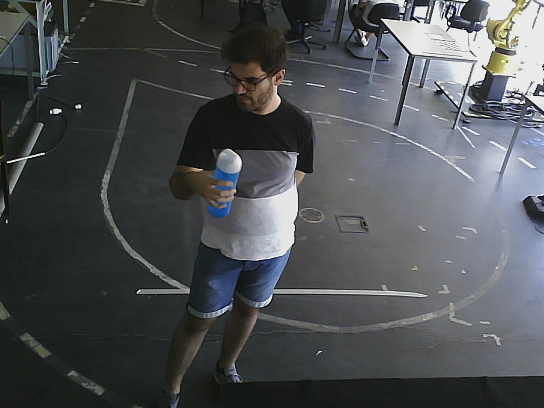
\includegraphics[width=0.4\textwidth]{figs/dataset_preprocessing1_1.png} \ 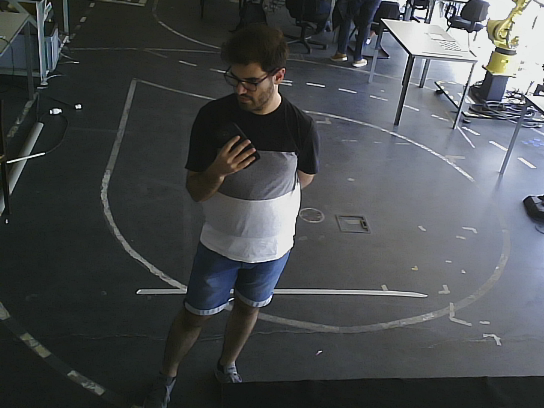
\includegraphics[width=0.4\textwidth]{figs/dataset_preprocessing1_2.png}}
    \caption{Dataset examples holding a bottle (left) and a phone (right).}
    \label{fig:dataset_examples}
\end{figure}

Naturally, the successive frames could lead to similar grasping patterns from different views. To investigate intra-user variability and to ensure robust model training, users are instructed to perform multiple grasping trials of the selected object across four distinct acquisition sessions. Bearing this in mind, the data acquisition system was designed to facilitate the fast generation of training datasets, accommodating the inclusion of new users and/or additional acquisition sessions. On the one hand, the system is integrated into the workflow of the proposed object recognition framework. On the other hand, it is particularly well-suited for implementation in industrial settings where end-users may not possess extensive expertise in machine learning or computer vision. The instructions provided to users during the data acquisition sessions were intentionally straightforward, ensuring that non-experts could readily participate in the process.

Videos over four sessions per user were recorded at 10 frames per second. For each object and each user, four data acquisition sessions were carried out, which gave rise to the dataset used in the study. Therefore, the dataset consists of a total of \num{11054} samples, distributed practically equally across the three participants (around \num{3600} samples per participant) and the four objects (between \num{2618} and \num{2849} samples per object). The exact number of samples of the entire dataset per class and per user is shown in \autoref{tab:dataset}.

\begin{table}[ht] 
\centering
\caption{Number of samples in the dataset per class and user}
\label{tab:dataset}
\begin{tabular}{lccccc}
\toprule
Dataset & Bottle & Cube & Phone & Screwdriver & Total \\
\midrule
User1 & \num{828} & \num{928} & \num{950} & \num{957} & \num{3663}\\
User2 & \num{886} & \num{926} & \num{939} & \num{946} & \num{3697}\\
User3 & \num{904} & \num{907} & \num{937} & \num{946} & \num{3694}\\
\midrule
Total & \num{2618} & \num{2761} & \num{2826} & \num{2849} & \num{11054}\\
\bottomrule
\end{tabular}
\end{table}

\subsubsection{Preprocessing}

After having a dataset, the data had to be processed to have a fitting structure to be used in the model training. The images from the videos were processed using the Mediapipe hands model resulting in 21 points for each hand detected (\autoref{fig:dataset_examples2}).

\begin{figure}[ht]
    \centerline{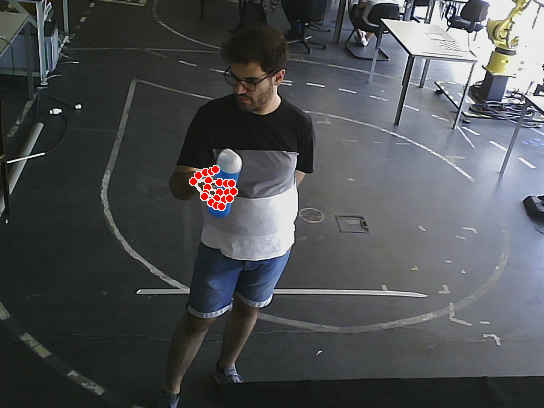
\includegraphics[width=0.4\textwidth]{figs/dataset_preprocessing2_1.png} \ 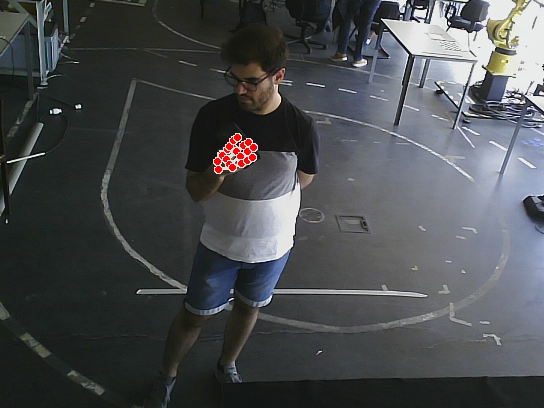
\includegraphics[width=0.4\textwidth]{figs/dataset_preprocessing2_2.png}}
    \caption{Points detected on the pictures in \autoref{fig:dataset_examples} by Mediapipe Hands Model.}
    \label{fig:dataset_examples2}
\end{figure}

The points corresponding to the right hand are then subject to further transformations and normalization. First, the original coordinates of the keypoints (raw data), which are already normalized within the range of 0 to 1 are converted into coordinates relative to a reference. Specifically, for each keypoint $P = (x,y,z)$, the coordinates of the reference point are subtracted $P_{ref} = (x_{ref}, y_{ref}, z_{ref})$ from them to obtain relative coordinates $P_{rel} = (x_{rel}, y_{rel}, z_{rel})$. In this study, the reference is defined as the centroid $C$ of the set of hand keypoints.
This transformation into relative coordinates is particularly useful because the absolute position of the hands in the image may vary from frame to frame due to different distances from the camera or hand orientations. Instead, relative coordinates are translation invariant and they reduce the influence of any rotations that might be present in the raw data. Therefore, the network will focus on the spatial relationships between keypoints, rather than their absolute positions, making it less sensitive to hand orientations and scale variations.

After obtaining the relative coordinates with respect to the reference point, scaling is applied to each dimension independently by dividing by an appropriate constant to ensure that the hand’s representation spans the entire range, as follows:
\begin{equation}
scaleFactor = \frac {0.5}{\max(\{\lvert x_i \rvert,\lvert y_i \rvert,\lvert z_i\rvert\}: i=1,\cdots,n)} \text{  ,}
\end{equation}
%
where $\{x_i,y_i,z_i\}$ denote relative coordinates. This feature scaling revealed to be a valuable pre-processing step to help make the data more consistent, helping the model to learn the relevant patterns without being influenced by variations in hand position, hand size, or scale. Further, it helps to maximize the separation among keypoints, helping the model to discriminate the output class. Finally, a uniform adjustment is made by adding 0.5 to each coordinate, centering the points between 0 and 1 on the scale. It is important to note that throughout the point processing, the order of the points is never changed, and therefore the models can take advantage of this structure. \autoref{fig:dataset_examples3} shows examples of the normalized keypoints representation expressed according to the previous steps, that is: 
\begin{equation}
P_{norm} = (P - C) \times scaleFactor + 0.5\text{ .}
\end{equation}

\begin{figure}[ht]
    \centerline{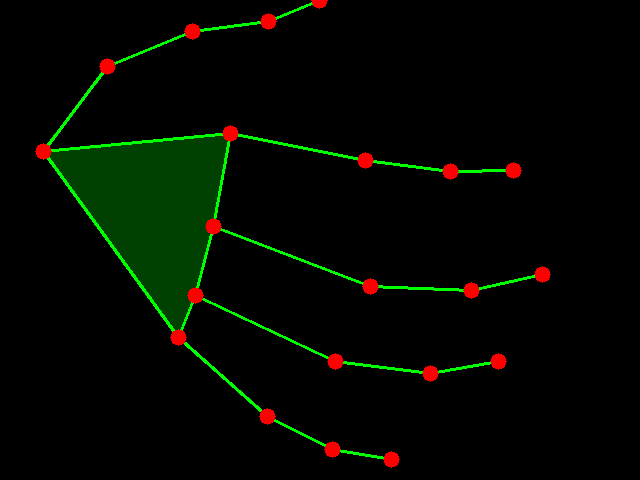
\includegraphics[width=0.4\textwidth]{figs/dataset_preprocessing3_1.png} \ 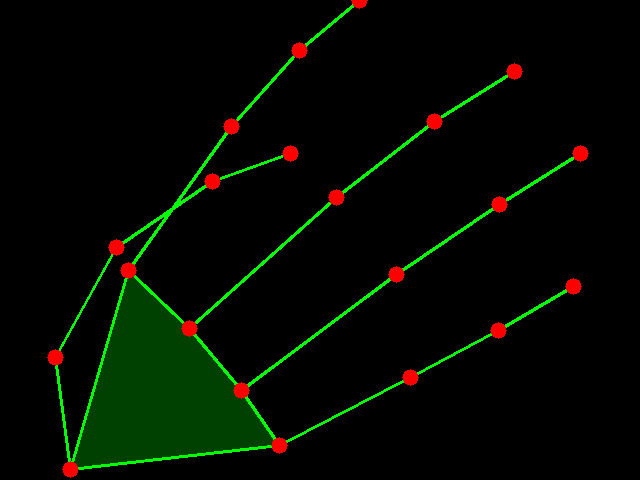
\includegraphics[width=0.4\textwidth]{figs/dataset_preprocessing3_2.png}}
    \caption{Points from the pictures in \autoref{fig:dataset_examples2} after normalization}
    \label{fig:dataset_examples3}
\end{figure}

\subsection{Models}

For this work, the architectures tested were the CNN and the Transformer given their ability at detecting local relations, which makes them an advantageous solution for this problem given that each sample provided to the model is made of the 21 3D points that always follow the same structure representing the right hand. \textcolor{red}{For further details... (cite article)}

\subsubsection{CNN Classifier}
\label{subsubsection:cnn_classifier}

The developed CNN comprises two convolutional layers each with 64 feature maps and ReLU activation functions. 
The first layer uses a kernel size of 3$\times$3 pixels performing a 1D convolution on the 3$\times$21 data with a stride of 1 pixel. The flattened output from the final layer is connected to a dense layer with 128 neurons, followed by another dense layer with the number of neurons equal to the number of classes. The output layer consists of the final connect layer with softmax activation. The softmax function takes a vector of real-valued scores (often called logits) and transforms them into a probability distribution over multiple classes. For the classification task with 4 classes, the output layer has 4 neurons, each representing the probability of the input belonging to a particular class. To prevent overfitting, dropout layers are incorporated after each fully connected layer. The final model can be seen in \autoref{fig:cnn_architecture} and it has \num{156644} trainable parameters. It is made of two convolutional layers followed by three dense layers, with the third being the output layer. Between the convolutional and the dense layers and between both dense layers, there is also a dropout layer to help with overfitting.

\begin{figure}[ht]
    \centering
    {\fontsize{9}{11}\selectfont\includesvg[width=\textwidth]{figs/cnn_architecture.svg}}
    \caption{CNN model architecture}
    \label{fig:cnn_architecture}
\end{figure}

\subsubsection{Transformer Neural Network Classifier}
\label{subsubsection:transformer_classifier}

The developed Transformer model is made of two Transformer encoder stacks (\autoref{fig:transformer_encoder_architecture}) comprised of the following layers: multi-head self-attention, layer normalization, and feedforward neural networks. Within each encoder, multi-head self-attention is applied to capture dependencies among the keypoints, where four attention heads are used for enhanced feature extraction. Following self-attention, two position-wise feedforward neural networks are employed to process the attended features and capture complex patterns. Layer normalization is applied after each sub-layer to stabilize the activations and facilitate training convergence. The resulting architecture can be seen in \autoref{fig:transformer_architecture} and it has \num{16384} trainable parameters.

\begin{figure}[H] %[ht]
    \centering
    {\fontsize{10}{12}\selectfont\includesvg[width=1\textwidth]{figs/transformer_encoder.svg}}
    \caption{Transformer encoder block}
    \label{fig:transformer_encoder_architecture}
\end{figure}

\begin{figure}[H] %[ht]
    \centering
    {\fontsize{10}{12}\selectfont\includesvg[width=1\textwidth]{figs/transformer_architecture.svg}}
    \caption{Transformer model architecture}
    \label{fig:transformer_architecture}
\end{figure}

\subsection{Model Comparison}

With both models trained, \autoref{table:model_comparison} shows the performance of all the machine learning models involved in this classification task, including those belonging to MediaPipe.

\begin{table}[H] %[ht]
    \centering
    \caption{Model Comparison}
    \label{table:model_comparison}
    \begin{tabular}{lcc}
        \toprule
        Model & Performance & Prediction Time (ms) \\
        \midrule
        Hand Landmarker & 10.09 MNAE* & 43.5 \\
        Pose Landmarker Lite & 87.0 PDJ* & 21.8 \\
        Pose Landmarker Full & 91.8 PDJ* & 28.7 \\
        Pose Landmarker Heavy & 94.2 PDJ* & 83.1 \\
        CNN Object Classifier & 90.5\% Acc* & 14.1 \\
        Transformer Object Classifier & 86.7\% Acc* & 16.0 \\
        \bottomrule
    \end{tabular}
    \captionsetup{width=0.9\textwidth}
    \caption*{*MNAE: Mean of Normalized Absolute Error\\ *PDJ: average Percentage of Detected Joints\\ *Acc: model Accuracy}
\end{table}

For the Hand Landmarker, there is only a single option available so it was the one used. Then, for the Pose Landmarker there are three options available but given that it has relatively less relevance and it runs in parallel with the Hand Landmarker, the Full version was used since it has the highest performance while keeping a lower prediction time. Finally, for the object classifier, the CNN presented the highest accuracy and the lowest prediction time so it was selected for further optimizations in real-time.

With all models of the pipeline selected, a test was made in real-time for each object to check the stability and reliability of the model prediction in a certain frame, resulting in the graphics in \autoref{fig:softmaxes}.

\begin{figure}[H]%[ht]
    \centering
    \begin{subfigure}[b]{0.8\columnwidth}
        {\fontsize{8}{10}\selectfont\includesvg[width=\textwidth]{figs/bottle_cnn_softmaxes.svg}}
        \caption{\centering}
        % \label{}
    \end{subfigure}
    \par\medskip
    \begin{subfigure}[b]{0.8\columnwidth}
        {\fontsize{8}{10}\selectfont\includesvg[width=\textwidth]{figs/cube_cnn_softmaxes.svg}}
        \caption{\centering}
        % \label{}
    \end{subfigure}
    \par\medskip
    \begin{subfigure}[b]{0.8\columnwidth}
        {\fontsize{8}{10}\selectfont\includesvg[width=\textwidth]{figs/plier_cnn_softmaxes.svg}}
        \caption{\centering}
        % \label{}
    \end{subfigure}
    \par\medskip
    \begin{subfigure}[b]{0.8\columnwidth}
        {\fontsize{8}{10}\selectfont\includesvg[width=\textwidth]{figs/screwdriver_cnn_softmaxes.svg}}
        \caption{\centering}
        % \label{}
    \end{subfigure}
    \caption{}
    \label{fig:softmaxes}
\end{figure}

These results show that there are a significant number of frames where the model outputs a softmax probability equal or very close to \num{1.0} about the wrong label, especially in the video where the user is holding a plier. Furthermore, these frames are not isolated, sometimes the error happens over multiple consecutive frames making it even harder to establish a rule about when a prediction is valid.

With the unreliability of the softmax probability, the values of the neural network before the softmax operation names logits were tested to ascertain if they would be able to provide additional information, resulting in the graphics in \autoref{fig:logits}.

\begin{figure}[H]%[ht]
    \centering
    \begin{subfigure}[b]{0.8\columnwidth}
        {\fontsize{8}{10}\selectfont\includesvg[width=\textwidth]{figs/bottle_cnn_logits.svg}}
        \caption{\centering}
        % \label{}
    \end{subfigure}
    \par\medskip
    \begin{subfigure}[b]{0.8\columnwidth}
        {\fontsize{8}{10}\selectfont\includesvg[width=\textwidth]{figs/cube_cnn_logits.svg}}
        \caption{\centering}
        % \label{}
    \end{subfigure}
    \par\medskip
    \begin{subfigure}[b]{0.8\columnwidth}
        {\fontsize{8}{10}\selectfont\includesvg[width=\textwidth]{figs/plier_cnn_logits.svg}}
        \caption{\centering}
        % \label{}
    \end{subfigure}
    \par\medskip
    \begin{subfigure}[b]{0.8\columnwidth}
        {\fontsize{8}{10}\selectfont\includesvg[width=\textwidth]{figs/screwdriver_cnn_logits.svg}}
        \caption{\centering}
        % \label{}
    \end{subfigure}
    \caption{}
    \label{fig:logits}
\end{figure}

The results show that across all four classes, when a logit value is higher than six, the model is always giving a correct prediction. This information can be used to create a rule that will only consider the prediction valid if the highest logit value is higher than six. As an extra layer of security, the prediction will only be considered valid if the model gives the same prediction for two consecutive frames. 
